\chapter{实验结果与分析}

本章旨在对前述章节设计并实现的动态可重构FPGA矩阵乘法加速系统进行全面的测试与评估。
我们将通过一系列实验来验证系统的功能正确性、测量动态重构的关键性能指标、
评估核心矩阵运算任务的加速效果(与CPU基准对比),并量化硬件资源的利用率。
本章的目标是提供实验证据,证明所提出设计的有效性和实用性。

\section{实验环境与配置}

实验硬件平台为Xilinx Kria KV260 Vision AI入门套件,
其核心是Zynq UltraScale+ MPSoC。使用的Vitis HLS与Vivado工具链版本均为2022.1。
可编程逻辑(PL)部分根据第四章所述的可重构模块设计,在综合实现后,各模块的工作时钟频率设定为250 MHz。
处理器系统(PS)端的ARM Cortex-A53四核处理器运行频率为1.33 GHz。
软件环境方面,KV260上部署了Xilinx特制的Ubuntu 22.04 LTS操作系统,
主机应用程序以及CPU基准程序(单线程的朴素矩阵乘法)均使用GCC 11.4.0进行编译,并开启 \verb|-O1| 优化。

\section{系统功能验证}

功能验证是确保系统按预期工作的首要步骤。我们针对第五章中描述的所有加速计算任务进行了测试:
稀疏矩阵解压为稠密矩阵、稠密矩阵压缩为稀疏矩阵、稀疏矩阵格式转换(例如,从假设的COO格式RM到CSR格式RM的转换流程)、
稠密矩阵乘法(结果分别为稠密和稀疏),以及稀疏矩阵乘法(结果分别为稠密和稀疏)。
实验结果表明,所有FPGA加速任务的输出均与CPU参考结果一致(在单精度浮点数允许的误差范围内),
从而验证了整个系统(包括HLS模块设计、AXI接口、XRT调用、DPR流程及主机应用程序逻辑)的功能正确性。

\section{GEMM加速性能分析}

我们对核心矩阵运算任务在FPGA上的加速性能进行了评估,并与纯CPU执行时间进行了对比。
性能指标主要关注端到端执行时间,即包括数据传输与FPGA内核执行的总时间。

对于稠密矩阵乘法 (GEMM),我们测试了128\texttimes{}128单精度浮点稠密矩阵乘法,FPGA上脉动阵列的每个块大小为12\texttimes{}12。
CPU执行时间约为32毫秒,而FPGA上的稠密矩阵乘法RM总共耗时1.3毫秒,实现了约25\texttimes{}的加速比。

\section{硬件资源利用率}

\begin{figure}[htbp]
\centerline{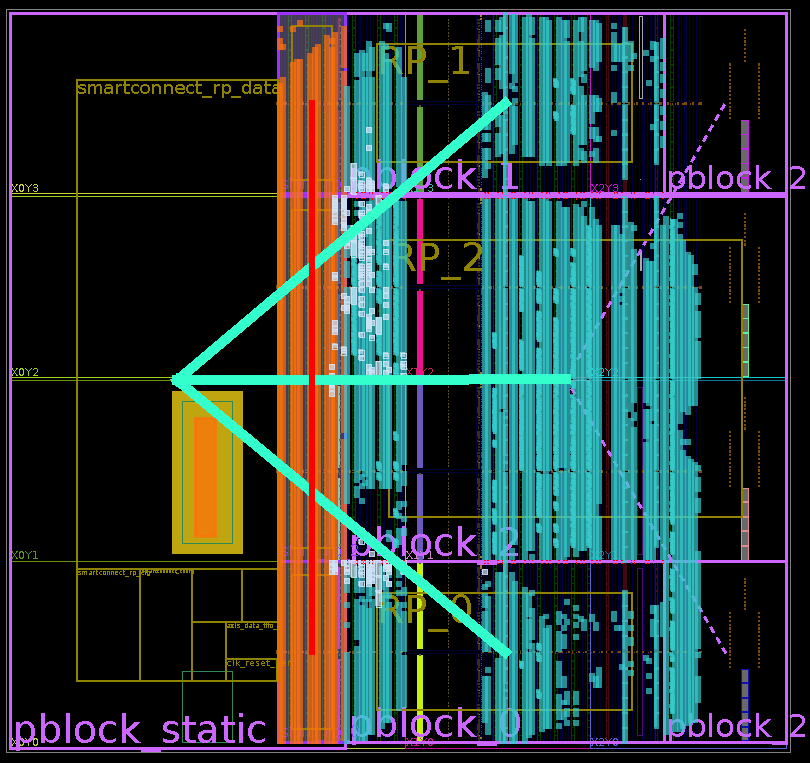
\includegraphics[width=0.8\columnwidth]{figures/a.png}}
\caption{FPGA实现。RP\_0上实现了COO矩阵解压RM,RP\_1上实现了COO矩阵压缩RM,RP\_2上实现了稠密矩阵乘法RM。}
\label{fig:a}
\end{figure}

\begin{figure}[htbp]
\centerline{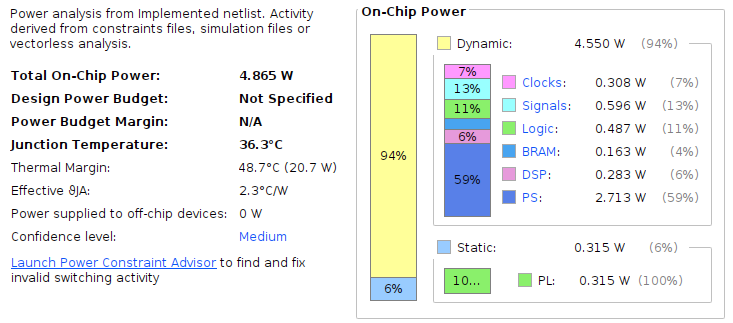
\includegraphics[width=0.8\columnwidth]{figures/b.png}}
\caption{能耗占用。}
\label{fig:b}
\end{figure}

\begin{figure}[htbp]
\centerline{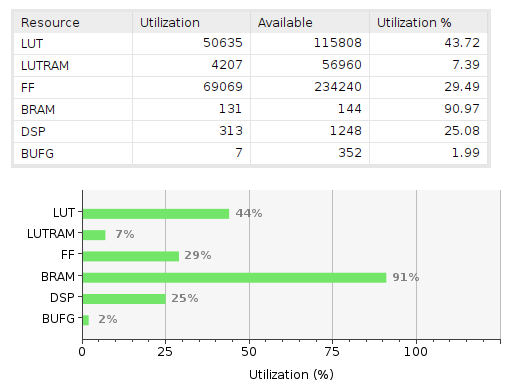
\includegraphics[width=0.8\columnwidth]{figures/c.png}}
\caption{资源利用。}
\label{fig:c}
\end{figure}

我们将COO矩阵解压、COO矩阵压缩以及稠密矩阵乘法作为一个整体,其在FPGA上的实现结果如图\ref{fig:a}所示,其能耗占用与资源利用分别由图\ref{fig:b}和图\ref{fig:c}所示。
可以看出,为支持128\texttimes{}128单精度浮点矩阵,我们几乎消耗了板上所有的BRAM。更大的矩阵规模将无法在这块KV260开发版上实现。
可以说,板上的全部资源都已被高效利用。如果增加分块脉动阵列的块大小,RP将无法在250 MHz的频率下运行。

\section{讨论与分析总结}

实验结果综合表明,所设计的动态可重构FPGA矩阵乘法加速系统成功实现了预期的功能,并在GEMM运算任务上展现了相对于ARM CPU的显著加速效果。
稠密矩阵乘法的脉动阵列设计和稀疏处理流水线的构建,有效地利用了FPGA的并行计算能力。动态部分重构机制虽然引入了一定的时间开销,
但其赋予系统的灵活性和适应性,使其能够高效应对多种计算需求和数据格式,这对于需要处理多样化任务的场景具有重要价值。
